\documentclass[tikz,border=5pt]{standalone}
\usepackage{amsmath}
\usetikzlibrary{arrows.meta,positioning,fit,calc}

\begin{document}
\pagecolor{white}
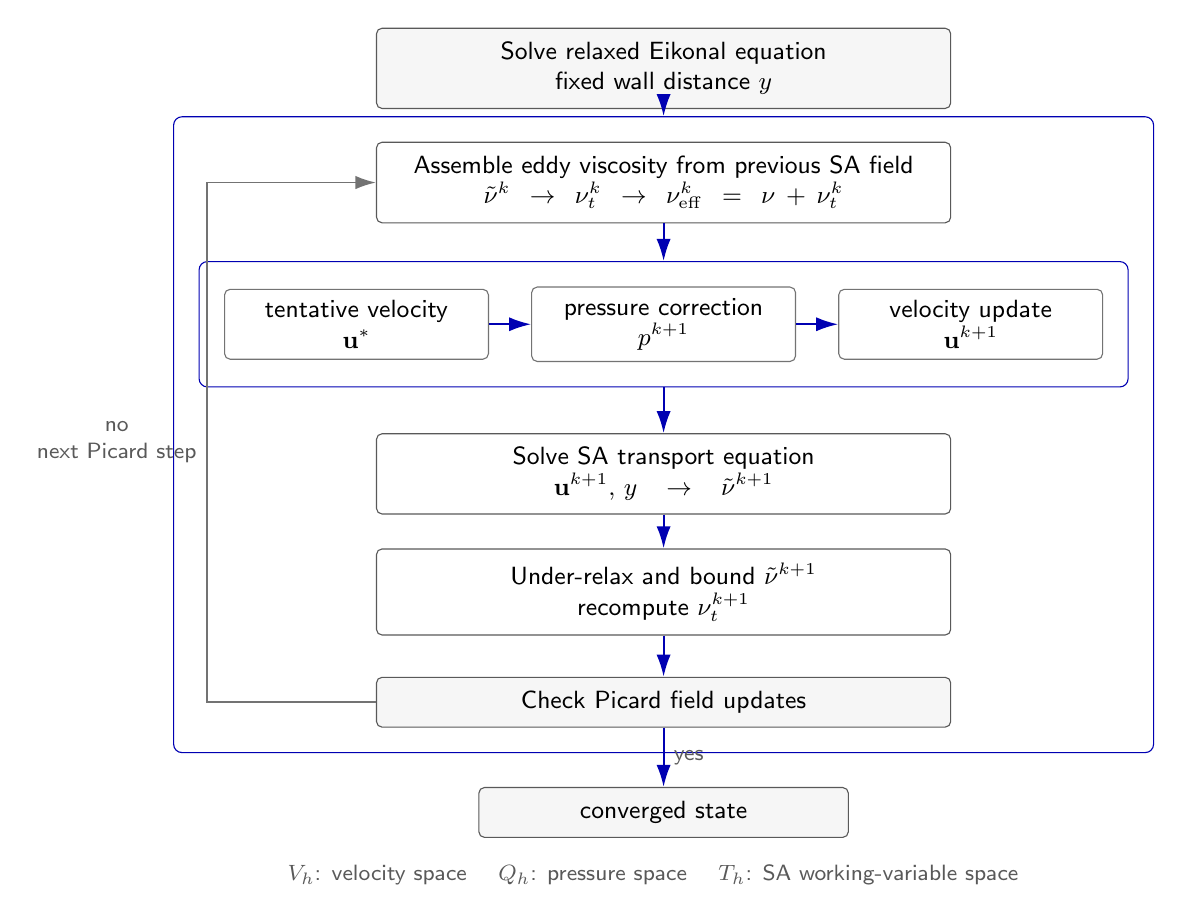
\begin{tikzpicture}[
    font=\sffamily\small,
    >=Latex,
    mainbox/.style={draw=black!65, rounded corners=2pt, fill=white,
                    align=center, inner xsep=7pt, inner ysep=5pt,
                    minimum width=72mm, text width=68mm},
    ipcstep/.style={draw=black!55, rounded corners=2pt, fill=white,
                    align=center, inner xsep=5pt, inner ysep=4pt,
                    minimum width=32mm, text width=30mm},
    group/.style={draw=blue!70!black, rounded corners=3pt,
                  inner xsep=9pt, inner ysep=9pt},
    arrow/.style={-{Latex[length=2.8mm,width=1.8mm]},
                  line width=0.75pt, draw=blue!70!black},
    returnarrow/.style={-{Latex[length=2.6mm,width=1.7mm]},
                        line width=0.65pt, draw=black!55},
    label/.style={font=\sffamily\footnotesize, text=black!65, align=center}
]

\node[mainbox, fill=gray!7] (eikonal) at (0,0)
    {Solve relaxed Eikonal equation\\fixed wall distance $y$};

\node[mainbox] (eddy) at (0,-1.45)
    {Assemble eddy viscosity from previous SA field\\
     $\tilde{\nu}^{k}\rightarrow \nu_t^{k}\rightarrow \nu_{\mathrm{eff}}^{k}=\nu+\nu_t^{k}$};

\node[ipcstep] (tent) at (-3.9,-3.25)
    {tentative velocity\\$\mathbf{u}^{*}$};
\node[ipcstep] (press) at (0,-3.25)
    {pressure correction\\$p^{k+1}$};
\node[ipcstep] (vel) at (3.9,-3.25)
    {velocity update\\$\mathbf{u}^{k+1}$};
\node[group, fit=(tent)(press)(vel), label={[label]above:IPCS velocity-pressure solve}] (ipcs) {};

\node[mainbox] (sa) at (0,-5.15)
    {Solve SA transport equation\\
     $\mathbf{u}^{k+1},\,y \rightarrow \tilde{\nu}^{k+1}$};

\node[mainbox] (relax) at (0,-6.65)
    {Under-relax and bound $\tilde{\nu}^{k+1}$\\
     recompute $\nu_t^{k+1}$};

\node[mainbox, fill=gray!7] (check) at (0,-8.05)
    {Check Picard field updates};

\node[group, fit=(eddy)(ipcs)(sa)(relax)(check),
      label={[font=\sffamily\bfseries\small,text=blue!70!black]north west:outer Picard iteration $k\rightarrow k+1$}] (picard) {};

\node[mainbox, fill=gray!7, minimum width=46mm, text width=42mm] (stop) at (0,-9.45)
    {converged state};

\draw[arrow] (eikonal) -- (picard.north);
\draw[arrow] (eddy) -- (ipcs.north);
\draw[arrow] (tent) -- (press);
\draw[arrow] (press) -- (vel);
\draw[arrow] (ipcs.south) -- (sa);
\draw[arrow] (sa) -- (relax);
\draw[arrow] (relax) -- (check);
\draw[arrow] (check) -- node[label, right] {yes} (stop);

\draw[returnarrow] (check.west) -- ++(-2.15,0)
    |- node[label, pos=0.25, left] {no\\next Picard step} (eddy.west);

\node[label, anchor=west] at (-4.9,-10.25)
    {$V_h$: velocity space \quad $Q_h$: pressure space \quad $T_h$: SA working-variable space};

\end{tikzpicture}
\end{document}
